\documentclass{article}


\usepackage{PRIMEarxiv}

\usepackage[utf8]{inputenc} % allow utf-8 input
\usepackage[T1]{fontenc}    % use 8-bit T1 fonts
\usepackage{hyperref}       % hyperlinks
\usepackage{url}            % simple URL typesetting
\usepackage{booktabs}       % professional-quality tables
\usepackage{amsfonts}       % blackboard math symbols
\usepackage{nicefrac}       % compact symbols for 1/2, etc.
\usepackage{microtype}      % microtypography
\usepackage{lipsum}
\usepackage{graphicx}
\usepackage{booktabs, multirow} 
\usepackage{amsmath,amssymb}
\DeclareMathOperator{\E}{\mathbb{E}}
\graphicspath{{media/}}     % organize your images and other figures under media/ folder


%% Title
\title{We Didn't Start The Fire: Robust Wildfire Detection With Limited Labeled Data}

\author{
  Ivanina Ivanova, Abhay Mathur \\
  Institut Polytechnique de Paris \\
  \texttt{\{abhay.mathur, ivanina.ivanova\}@ip-paris.fr} \\
  %% examples of more authors
}


\begin{document}
\maketitle

% \begin{abstract}
% \end{abstract}

\section{Problem Statement}
This project aims to develop a fire detection system using a designated
dataset. The dataset consists of three subsets: a training set, a validation
set, and a test set. Specific constraints and guidelines must be strictly
followed to ensure compliance with the project requirements.

\subsection{Dataset Access and Constraints}

The dataset is available for download at
\url{https://www.kaggle.com/datasets/abdelghaniaaba/wildfire-prediction-dataset/code}.
It comprises a training set, a validation set, and a test set. A critical
restriction is imposed on the training set: its labels are inaccessible. Any
direct utilization of annotations from the training set will lead to
disqualification.

\subsection{Dataset Partitioning}

To facilitate model training, the original validation set must be partitioned
into a newly defined validation set and a new training set. The original
training set may be leveraged in a creative manner; however, its labels must
not be employed under any circumstances.

\subsection{Model Development}

A deep neural network (DNN) will be trained utilizing the newly defined
training and validation sets. Various methodologies and supplementary resources
may be incorporated to enhance model performance, provided that all constraints
related to annotation usage are rigorously upheld.

\section{Dataset Analysis}

\begin{figure}
  \centering
  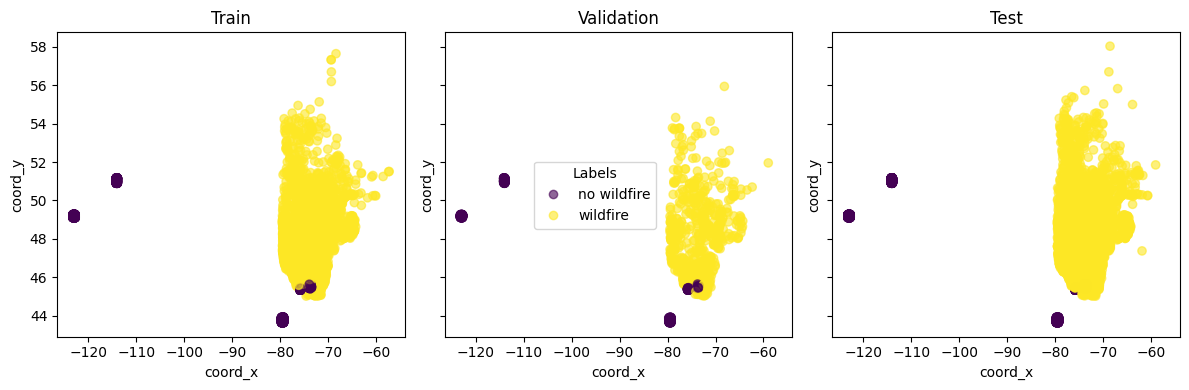
\includegraphics[width=0.8\textwidth]{figures/coord_label.png}
  \caption{Spatial Distribution of the Dataset. All splits show a similar spread of zones where fires are detected.}
  \label{fig:dataset_analysis}
\end{figure}

\section{Baselines: Using Available Labeled Data}

\subsubsection{Naive Coordinates Classifier}
\dots

\subsubsection{Image Classifiers}
\dots

\subsubsection{Fused Classifiers}
\dots

\section{Self-Supervision (Learning from Unlabeled Data)}

\subsection{SimCLR}
SimCLR (Simple Framework for Contrastive Learning of Visual Representations) is
a self-supervised learning method that does not require any labels. It learns
visual representations by maximizing the agreement between differently
augmented views of the same data example.

The training pipeline of SimCLR consists of the following steps:

\subsubsection{Data Augmentation}
Each input image is transformed into two different augmented views through a
series of random augmentations such as cropping, resizing, flipping, color
jittering, and Gaussian blurring. These augmentations are crucial as they
create diverse views of the same image, which the model learns to recognize as
similar.

\subsubsection{Encoder Network}
Both augmented views are passed through an encoder network (typically a ResNet)
to obtain their respective feature representations. The encoder network is
shared between the two views.

\subsubsection{Projection Head}
The feature representations are then passed through a small neural network
called the projection head, which maps them to a latent space where the
contrastive loss is applied. The projection head typically consists of a few
fully connected layers.

\subsubsection{Contrastive Loss}
The core idea of SimCLR is to bring the representations of the two augmented
views of the same image closer together in the latent space while pushing apart
representations of different images. This is achieved using a contrastive loss
function, specifically the normalized temperature-scaled cross-entropy loss
(NT-Xent loss). The loss function is defined as:

\begin{align}
  \mathcal{L}_{i,j} & = -\log
  \frac{\exp(\text{sim}(\mathbf{z}_i, \mathbf{z}_j) / \tau)}{\sum_{k=1}^{2N}
  \mathbb{1}_{[k \neq i]} \exp(\text{sim}(\mathbf{z}_i, \mathbf{z}_k) / \tau)}
\end{align}

Where $\mathbf{z}_i$ and $\mathbf{z}_j$ are the latent representations of the
two augmented views of the same image, $\text{sim}(\cdot, \cdot)$ denotes the
cosine similarity, $\tau$ is a temperature parameter, and $N$ is the batch
size.

By training the model in this manner, SimCLR learns robust and generalizable
visual representations that can be fine-tuned for downstream tasks such as
classification, even with limited labeled data.

Just wanted to cite this paper~\cite{simclr}.

\subsection{Variational Autoencoder (VAE) + Classifier}

A Variational Autoencoder (VAE) was employed as a self-supervised learning
approach to extract latent representations from the training dataset. The VAE
comprises an encoder network, which maps input images to a latent space
distribution, and a decoder network, which reconstructs the input from latent
variables. The encoder network consists of a series of 4 convolutional layers
followed by fully connected layers, while the decoder network mirrors the
encoder architecture. The VAE was trained using the unlabeled training dataset.
The training objective that we decided to use is Beta-VAE~\cite{beta-vae}.
Beta-VAE is a modification of the original VAE that introduces a hyperparameter
$\beta$ to the loss function. The $\beta$ parameter controls the trade-off
between the reconstruction loss and the Kullback-Leibler divergence. The loss
function for the Beta-VAE is given by:

\begin{align}
  \mathcal{L}(\theta, \phi, x, z, \beta) & = \E_{q_\phi(z|x)}[\log p_\theta(x|z)] - \beta D_{KL}(q_\phi(z|x)\| p(z))
\end{align}

where $p(z|x)$ is the learned posterior, $p(z)$ is the prior distribution
(assumed to be Gaussian), and $p(x|z$) represents the likelihood of
reconstructing the input image from the latent space. Well chosen $\beta$
values can lead to disentangled representations in the latent space. The VAE
was trained for 50 epochs using the Adam optimizer with a learning rate of
0.0001. The latent representations obtained from the VAE were then used to
train a classifier. The classifier consists of a two fully connected layer with
a ReLU activation fucntion and a Dropout layer in between. The classifier was
trained using the labeled train dataset. The training objective was to minimize
the binary cross-entropy loss between the predicted and true labels. The linear
classifier was trained for 20 epochs using the Adam optimizer with a learning
rate of 0.0001.

\begin{table}[!htp]\centering
  \caption{Results of different models with and without pre-training.}\label{tab:global_results}
  \scriptsize
  \begin{tabular}{cllccc}\toprule
    \textbf{Pre-Training}             & \textbf{Model}                                   & \textbf{Backbone}           & \textbf{\#params} & \textbf{Accuracy} & \textbf{F1 Score} \\ \cmidrule{1-6}
    ---                               & Coordinate Classifier                            & ---                         & \textbf{4.417K}   & 0.855             & 0.873             \\ \cmidrule{1-6}
    ---                               & CNN                                              & ---                         & 14.912M           & 0.9446            & 0.9491            \\ \cmidrule{1-6}
    ---                               & CNN + Coordinate Classifier                      & ---                         & 14.913M           & 0.9832            & 0.9849            \\ \cmidrule{1-6}
    \multirow{4}{*}{---}              & \multirow{4}{*}{Feature Classifier}              & ResNet18                    & 11.441M           & 0.983             & 0.984             \\
                                      &                                                  & ResNet34                    & 21.549M           & 0.98              & 0.982             \\
                                      &                                                  & ResNet50                    & 27.711M           & 0.985             & 0.986             \\
                                      &                                                  & ResNet101                   & 46.703M           & 0.978             & 0.98              \\ \cmidrule{1-6}
    \multirow{4}{*}{---}              & \multirow{4}{*}{Feature + Coordinate Classifier} & ResNet18                    & 11.442M           & 0.9916            & 0.9924            \\
                                      &                                                  & ResNet34                    & 21.550M           & \textbf{0.9921}   & \textbf{0.9928}   \\
                                      &                                                  & ResNet50                    & 24.560M           & 0.9906            & 0.9915            \\
                                      &                                                  & ResNet101                   & 43.552M           & 0.99              & 0.991             \\ \cmidrule{1-6}
    \multirow{4}{*}{SimCLR}           & \multirow{4}{*}{Feature Classifier}              & ResNet18                    & 11.523M           &                   &                   \\
                                      &                                                  & ResNet34                    & 21.631M           &                   &                   \\
                                      &                                                  & ResNet50                    & 27.988M           & 0.982             & 0.983             \\
                                      &                                                  & ResNet101                   & 46.980M           &                   &                   \\ \cmidrule{1-6}
    \multirow{2}{*}{Pseudo Labelling} & CNN                                              & ---                         & 14.912M           & 0.971             & 0.9737            \\
                                      & CNN+Coordinate Classifier                        & ---                         & 14.913M           & 0.9867            & 0.9879            \\\cmidrule{1-6}
    \multirow{4}{*}{$\beta$-VAE}      & \multirow{4}{*}{Feature Classifier}              & \#layers = 5                &                   & 0.887             & 0.9               \\
                                      &                                                  & \& coords                   &                   & 0.936             & 0.943             \\
                                      &                                                  & ResNet18          \& coords &                   & 0.934             & 0.942             \\
                                      &                                                  & ResNet50          \& coords &                   & 0.915             & 0.926             \\ \cmidrule{1-6}
    \multirow{2}{*}{VQ-VAE}           & \multirow{2}{*}{Feature Classifier}              & \& coords                   &                   & 0.931             & 0.936             \\
                                      &                                                  & ResNet50          \& coords &                   & 0.959             & 0.968             \\ \midrule
    \bottomrule
  \end{tabular}
\end{table}

\section{Experiments and Results}

\section{Conclusion}
Your conclusion here

%Bibliography
\bibliographystyle{unsrt}
\bibliography{references}

\end{document}
